\documentclass[letter,12pt]{article}
\usepackage[paperheight=27.94cm,paperwidth=21.59cm,bindingoffset=0in,left=3cm,right=2.0cm, top=3.5cm,bottom=2.5cm, headheight=200pt, headsep=1.0\baselineskip]{geometry}
\usepackage{graphicx,lastpage}
\usepackage{upgreek}
\usepackage{censor}
\usepackage[spanish,es-tabla]{babel}
\usepackage{pdfpages}
\usepackage{tabularx}
\usepackage{graphicx}
\usepackage{adjustbox}
\usepackage{xcolor}
\usepackage{colortbl}
\usepackage{rotating}
\usepackage{multirow}
\usepackage[T1]{fontenc}
\usepackage[utf8]{inputenc}
\usepackage{float}
\usepackage{hyperref}
\usepackage{subcaption}
\usepackage{listings}

\lstset{
    basicstyle=\ttfamily\small,
    breaklines=true,
    frame=single,
    language=Python,
    showstringspaces=false,
    numbers=left,
    numberstyle=\tiny,
    keywordstyle=\color{blue},
    commentstyle=\color{gray},
    stringstyle=\color{red}
}

\renewcommand{\tablename}{Tabla}
\usepackage{fancyhdr}
\pagestyle{fancy}

\fancyhead[L]{}
%
\begin{document}
%
   \title{\Huge{Informe Laboratorio 4}}

   \author{\textbf{Sección 1} \\  \\Alumno Felipe Maturana Araya \\ e-mail: felipe.maturana1@mail.udp.cl}
          
   \date{Mayo de 2026}

   \maketitle
   
   \tableofcontents
 
  \newpage
  

\section{Descripción de actividades}
Desarrollar un programa en Python utilizando la librería pycryptodome para cifrar y descifrar mensajes con los algoritmos DES, AES-256 y 3DES, permitiendo la entrada de la key, vector de inicialización y el texto a cifrar desde la terminal. 

Instrucciones:

\begin{enumerate}
    \item Investigación
    \begin{itemize}
        \item Investigue y documente el tamaño en bytes de la clave y el vector de inicialización (IV) requeridos para los algoritmos DES, AES-256 y 3DES. Mencione las principales diferencias entre cada algoritmo, sea breve.
    \end{itemize}

    \item El programa debe solicitar al usuario los siguientes datos desde la terminal
    \begin{itemize}
        \item Key correspondiente a cada algoritmo.
        \item Vector de Inicialización (IV) para cada algoritmo.
        \item Texto a cifrar.
    \end{itemize}

    \item Validación y ajuste de la clave
    \begin{itemize}
        \item Si la clave ingresada es menor que el tamaño necesario para el algoritmo complete los bytes faltantes agregando bytes adicionales generados de manera aleatoria (utiliza get\_random\_bytes).
        \item Si la clave ingresada es mayor que el tamaño requerido, trunque la clave a la longitud necesaria.
        \item Imprima la clave final utilizada para cada algoritmo después de los ajustes.
    \end{itemize}

    \item Cifrado y Descifrado
    \begin{itemize}
        \item Implemente una función para cada algoritmo de cifrado y descifrado (DES, AES-256, y 3DES). Use el modo CBC para todos los algoritmos.
        \item Asegúrese de utilizar el IV proporcionado por el usuario para el proceso de cifrado y descifrado.
        \item Imprima tanto el texto cifrado como el texto descifrado.
    \end{itemize}

    \item Comparación con un servicio de cifrado online
    \begin{itemize}
        \item Selecciona uno de los tres algoritmos (DES, AES-256 o 3DES), ingrese el mismo texto, key y vector de inicialización en una página web de cifrado online.
        \item Compare los resultados de tu programa con los del servicio online. Valide si el resultado es el mismo y fundamente su respuesta.
    \end{itemize}

    \item Aplicabilidad en la vida real
    \begin{itemize}
        \item Describa un caso, situación o problema donde usaría cifrado simétrico. Defina que algoritmo de cifrado simétrico recomendaría justificando su respuesta.
        \item Suponga que la recomendación que usted entrego no fue bien percibida por su contraparte y le pide implementar hashes en vez de cifrado simétrico. Argumente cuál sería su respuesta frente a dicha solicitud. 
    \end{itemize}
\end{enumerate}



\section{Desarrollo de actividades según criterio de rúbrica}

\subsection{Investiga y documenta los tamaños de clave e IV}

Los algoritmos de cifrado simétrico DES, AES-256 y 3DES requieren tamaños específicos de clave y vector de inicialización (IV) para operar correctamente. A continuación se documentan estos valores según las especificaciones del NIST.

\subsubsection*{DES (Data Encryption Standard)}
Según la especificación FIPS 46-3 \cite{nist_fips46}, DES utiliza una clave de 64 bits (8 bytes), de los cuales solo 56 bits son efectivos ya que los 8 bits restantes se usan para paridad. El tamaño de bloque es de 64 bits, por lo que el IV en modo CBC debe ser de 8 bytes \cite{dworkin2001}.

\subsubsection*{AES-256 (Advanced Encryption Standard)}
El estándar FIPS 197 \cite{nist_fips197} define que AES-256 utiliza una clave de 256 bits (32 bytes). El tamaño de bloque de AES es fijo en 128 bits (16 bytes) para todas las variantes (128, 192 y 256 bits de clave). En modo CBC, el IV debe coincidir con el tamaño de bloque, es decir, 16 bytes \cite{dworkin2001}.

\subsubsection*{3DES (Triple DES)}
Según NIST SP 800-67 \cite{nist_sp800_67}, 3DES aplica el algoritmo DES tres veces consecutivas. La clave total es de 192 bits (24 bytes), compuesta por tres claves DES de 64 bits cada una (con 56 bits efectivos por clave, dando 168 bits de seguridad nominal). El tamaño de bloque es el mismo que DES: 64 bits, por lo que el IV en modo CBC es de 8 bytes \cite{dworkin2001}.

\subsubsection*{Principales diferencias}

\begin{itemize}
    \item \textbf{Seguridad:} DES es considerado inseguro desde hace años debido a su clave corta de 56 bits. 3DES mejoró la seguridad aplicando DES tres veces, pero también fue retirado por NIST en 2024. AES-256 es el estándar vigente recomendado por NIST \cite{nist_fips197}.
    \item \textbf{Rendimiento:} AES es más rápido que 3DES, ya que 3DES ejecuta DES tres veces sobre cada bloque. Además, AES fue diseñado para ser eficiente tanto en hardware como en software \cite{nist_fips197}.
    \item \textbf{Tamaño de bloque:} DES y 3DES operan con bloques de 64 bits, mientras que AES trabaja con bloques de 128 bits, lo que le da mayor resistencia contra ciertos ataques \cite{dworkin2001}.
\end{itemize}

\clearpage

\subsection{Solicita datos de entrada desde la terminal}

El programa solicita tres datos al usuario mediante la función \texttt{input()} de Python: la clave (key), el vector de inicialización (IV) y el texto a cifrar. Estos valores se ingresan como cadenas de texto y luego se convierten a bytes con codificación UTF-8 para ser procesados por los algoritmos.

El siguiente fragmento muestra cómo se solicitan los datos:

\begin{lstlisting}
key_input = input("\nIngrese la clave (key): ")
iv_input  = input("Ingrese el vector de inicializacion (IV): ")
texto     = input("Ingrese el texto a cifrar: ")

key_bytes   = key_input.encode("utf-8")
iv_bytes    = iv_input.encode("utf-8")
texto_bytes = texto.encode("utf-8")
\end{lstlisting}

La Figura \ref{fig:entrada_datos} muestra la ejecución del programa en la terminal donde se ingresan los tres valores solicitados.

\begin{figure}[H]
    \centering
    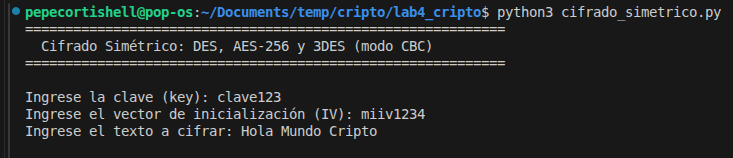
\includegraphics[width=0.9\textwidth,keepaspectratio]{img/entrada_datos.png}
    \caption{Ingreso de datos desde la terminal: clave, IV y texto a cifrar.}
    \label{fig:entrada_datos}
\end{figure}

\clearpage

\subsection{Valida y ajusta la clave según el algoritmo}

El programa implementa una función llamada \texttt{ajustar\_clave()} que recibe la clave ingresada, el tamaño requerido por el algoritmo y el nombre del algoritmo. La lógica es la siguiente:

\begin{itemize}
    \item Si la clave es \textbf{menor} al tamaño requerido, se completan los bytes faltantes con bytes aleatorios generados mediante \texttt{get\_random\_bytes()}.
    \item Si la clave es \textbf{mayor} al tamaño requerido, se trunca a la longitud necesaria.
    \item Si la clave tiene el \textbf{tamaño exacto}, se usa tal cual.
\end{itemize}

El fragmento de código correspondiente es:

\begin{lstlisting}
def ajustar_clave(key_bytes, tam_requerido, nombre_algo):
    if len(key_bytes) < tam_requerido:
        relleno = get_random_bytes(tam_requerido - len(key_bytes))
        key_bytes = key_bytes + relleno
    elif len(key_bytes) > tam_requerido:
        key_bytes = key_bytes[:tam_requerido]
    return key_bytes
\end{lstlisting}

Después del ajuste, se imprime la clave final en formato hexadecimal para cada algoritmo. Las Figuras \ref{fig:ajuste_clave1} y \ref{fig:ajuste_clave2} muestran los dos tipos de respuesta que genera el programa según el tamaño de la clave ingresada.

\begin{figure}[H]
    \centering
    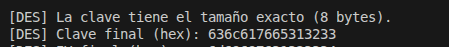
\includegraphics[width=0.9\textwidth,keepaspectratio]{img/ajuste_clave1.png}
    \caption{Caso donde la clave ingresada tiene el tamaño exacto requerido por el algoritmo.}
    \label{fig:ajuste_clave1}
\end{figure}

\begin{figure}[H]
    \centering
    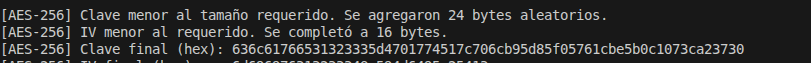
\includegraphics[width=0.9\textwidth,keepaspectratio]{img/ajuste_clave2.png}
    \caption{Caso donde la clave es menor al tamaño requerido y se completa con bytes aleatorios.}
    \label{fig:ajuste_clave2}
\end{figure}

\clearpage

\subsection{Implementa el cifrado y descifrado en modo CBC}

Se implementaron funciones separadas para cifrar y descifrar con cada algoritmo (DES, AES-256 y 3DES), todas utilizando el modo CBC. Se utiliza padding PKCS7 mediante las funciones \texttt{pad()} y \texttt{unpad()} de pycryptodome, ya que CBC requiere que el texto sea múltiplo del tamaño de bloque.

A continuación se muestra como ejemplo la función de cifrado y descifrado para AES-256:

\begin{lstlisting}
def cifrar_aes256(texto, key, iv):
    cipher = AES.new(key, AES.MODE_CBC, iv)
    ct = cipher.encrypt(pad(texto, AES.block_size))
    return ct

def descifrar_aes256(ct, key, iv):
    cipher = AES.new(key, AES.MODE_CBC, iv)
    pt = unpad(cipher.decrypt(ct), AES.block_size)
    return pt
\end{lstlisting}

Las funciones para DES y 3DES siguen la misma estructura, cambiando únicamente el módulo (\texttt{DES}, \texttt{DES3}) y el tamaño de bloque correspondiente.

El programa imprime para cada algoritmo: la clave final utilizada, el IV, el texto cifrado en hexadecimal, el texto descifrado y una verificación de que el texto descifrado coincide con el original.

La Figura \ref{fig:cifrado_des} muestra los resultados del cifrado y descifrado con DES.

\begin{figure}[H]
    \centering
    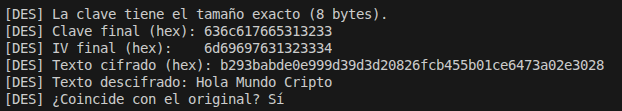
\includegraphics[width=0.9\textwidth,keepaspectratio]{img/cifrado_des.png}
    \caption{Resultado del cifrado y descifrado con DES en modo CBC.}
    \label{fig:cifrado_des}
\end{figure}

La Figura \ref{fig:cifrado_aes} muestra los resultados para AES-256.

\begin{figure}[H]
    \centering
    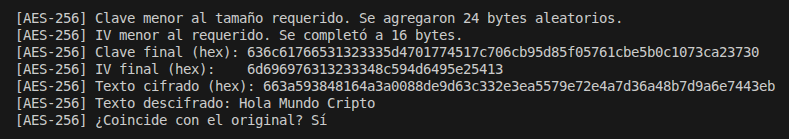
\includegraphics[width=0.9\textwidth,keepaspectratio]{img/cifrado_aes.png}
    \caption{Resultado del cifrado y descifrado con AES-256 en modo CBC.}
    \label{fig:cifrado_aes}
\end{figure}

La Figura \ref{fig:cifrado_3des} muestra los resultados para 3DES.

\begin{figure}[H]
    \centering
    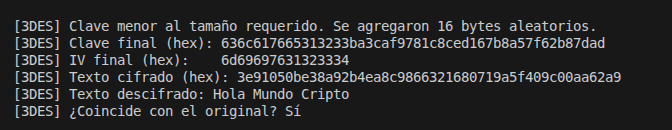
\includegraphics[width=0.9\textwidth,keepaspectratio]{img/cifrado_3des.png}
    \caption{Resultado del cifrado y descifrado con 3DES en modo CBC.}
    \label{fig:cifrado_3des}
\end{figure}

Finalmente, la Figura \ref{fig:ejecucion_completa} muestra una ejecución completa del programa con los tres algoritmos, donde se verifica que el texto descifrado coincide con el original en todos los casos.

\begin{figure}[H]
    \centering
    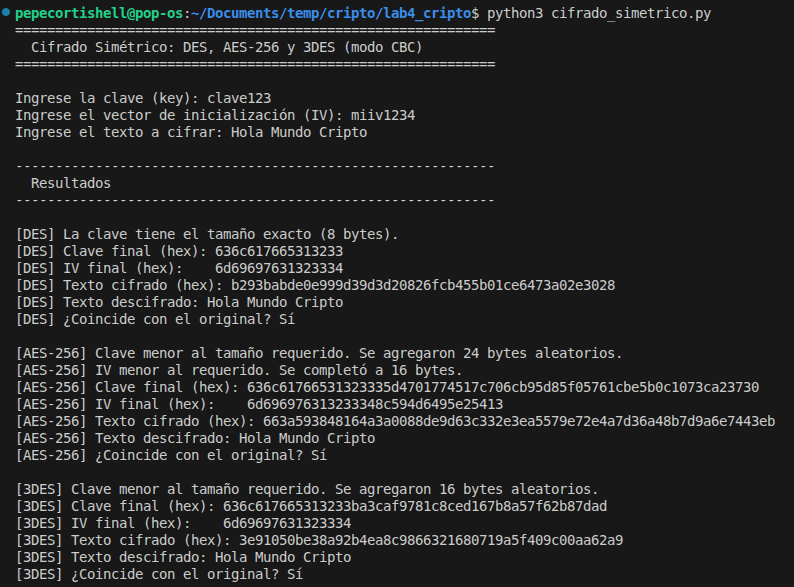
\includegraphics[width=0.9\textwidth,keepaspectratio]{img/ejecucion_completa.png}
    \caption{Ejecución completa del programa mostrando los tres algoritmos.}
    \label{fig:ejecucion_completa}
\end{figure}

\clearpage

\subsection{Compara los resultados con un servicio de cifrado online}

Para validar los resultados del programa, se seleccionó el algoritmo DES y se utilizó la herramienta online The-X Cryptography \cite{thex_des}. Se ingresaron los mismos parámetros: clave \texttt{clave123}, IV \texttt{miiv1234}, texto \texttt{Hola Mundo Cripto}, modo CBC y padding PKCS7.

La Figura \ref{fig:online_config} muestra la configuración utilizada en la herramienta online.

\begin{figure}[H]
    \centering
    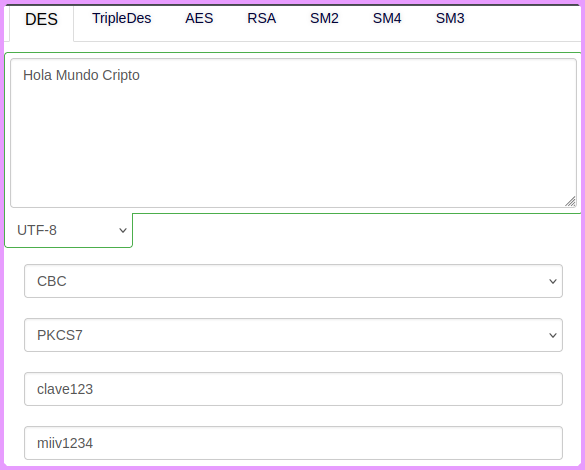
\includegraphics[width=0.9\textwidth,keepaspectratio]{img/online_config.png}
    \caption{Configuración del cifrado DES-CBC en la herramienta online \cite{thex_des}.}
    \label{fig:online_config}
\end{figure}

La Figura \ref{fig:online_resultado} muestra el resultado obtenido por el servicio online.

\begin{figure}[H]
    \centering
    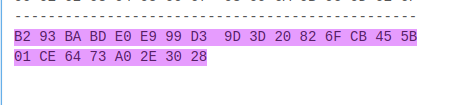
\includegraphics[width=0.9\textwidth,keepaspectratio]{img/online_resultado.png}
    \caption{Resultado del cifrado online con los mismos parámetros.}
    \label{fig:online_resultado}
\end{figure}

Para que ambos resultados coincidan, es necesario que se utilicen exactamente los mismos parámetros: algoritmo, modo de operación, clave, IV y padding. Si alguno difiere, el texto cifrado será completamente distinto. En caso de no coincidir, la causa más común es una diferencia en la codificación de la clave o el IV (por ejemplo, texto UTF-8 versus hexadecimal) o en el tipo de padding.

\clearpage

\subsection{Describe la aplicabilidad del cifrado simétrico en la vida real}

\subsubsection*{Caso de uso: Protección de registros médicos}

Un escenario real donde se aplica cifrado simétrico es la protección de fichas médicas en centros de salud. La normativa HIPAA del Departamento de Salud de Estados Unidos establece que los datos electrónicos de pacientes deben ser cifrados para considerarse protegidos ante una filtración \cite{hhs_hipaa}. El estándar recomendado para datos en reposo es AES-256, ya que es el algoritmo vigente aprobado por NIST, ofrece una clave de 256 bits resistente a fuerza bruta y tiene buen rendimiento para archivos grandes. DES y 3DES no son opciones viables porque ya fueron retirados por NIST.

El funcionamiento sería sencillo: cuando se guarda una ficha, el sistema la cifra con AES-256 usando una clave almacenada de forma segura. Cuando un médico necesita leerla, el sistema la descifra temporalmente.

\subsubsection*{Respuesta ante la solicitud de usar hashes}

No sería posible reemplazar cifrado simétrico por hashing. Un hash es una operación de una sola vía que genera un resumen fijo a partir de un dato, pero no permite recuperar el dato original. Sirve para verificar integridad o almacenar contraseñas, no para proteger información que necesita ser leída después. El cifrado simétrico sí es reversible: se cifra con una clave y se descifra con la misma. En el caso de las fichas médicas, los médicos necesitan leer el contenido, así que es obligatorio poder descifrar. Si se aplicara un hash, los datos se perderían.

\section*{Conclusiones y comentarios}

En este laboratorio se implementó un programa en Python capaz de cifrar y descifrar mensajes con DES, AES-256 y 3DES en modo CBC. Se pudo comprobar que los tres algoritmos producen un texto cifrado que, al ser descifrado con la misma clave e IV, devuelve el texto original sin alteraciones. Además, se validó el ajuste automático de claves cuando el usuario ingresa una clave de tamaño incorrecto, lo cual es un aspecto importante en la práctica.

La comparación con un servicio online permitió verificar que, si se utilizan los mismos parámetros (clave, IV, modo y padding), los resultados deben coincidir. Esto refuerza que los algoritmos de cifrado son determinísticos: con las mismas entradas, siempre producen la misma salida. También quedó claro que AES-256 es el algoritmo más recomendable actualmente, ya que DES y 3DES fueron retirados por NIST debido a vulnerabilidades en el tamaño de clave y bloque.

\begin{thebibliography}{9}

\bibitem{nist_fips46}
National Institute of Standards and Technology. (1999). \textit{Data Encryption Standard (DES)} (FIPS PUB 46-3). U.S. Department of Commerce. \url{https://csrc.nist.gov/publications/detail/fips/46/3/archive/1999-10-25}

\bibitem{nist_fips197}
National Institute of Standards and Technology. (2001). \textit{Advanced Encryption Standard (AES)} (FIPS PUB 197). U.S. Department of Commerce. \url{https://csrc.nist.gov/publications/detail/fips/197/final}

\bibitem{nist_sp800_67}
Barker, W. y Barker, E. (2012). \textit{Recommendation for the Triple Data Encryption Algorithm (TDEA) Block Cipher} (NIST SP 800-67 Rev. 2). National Institute of Standards and Technology. \url{https://csrc.nist.gov/publications/detail/sp/800-67/rev-2/final}

\bibitem{dworkin2001}
Dworkin, M. (2001). \textit{Recommendation for Block Cipher Modes of Operation: Methods and Techniques} (NIST SP 800-38A). National Institute of Standards and Technology. \url{https://csrc.nist.gov/publications/detail/sp/800-38a/final}

\bibitem{hhs_hipaa}
U.S. Department of Health and Human Services. (2013). \textit{HIPAA Security Rule: Technical Safeguards} (45 CFR §164.312). \url{https://www.hhs.gov/hipaa/for-professionals/security/laws-regulations/index.html}

\bibitem{thex_des}
The-X.cn. (s.f.). \textit{DES Encrypt/Decrypt Online Tool}. Recuperado el 29 de mayo de 2025, de \url{https://the-x.cn/en-us/cryptography/Des.aspx}

\end{thebibliography}

\end{document}
